\section{Методика}

	Суть работы заключается в анализе данных наблюдения за рентгеновскими пульсарами и кандидатами в черные дыры с космических аппаратов, дальнейшее определение параметров таких особенностей компактных объектов, как квазипериодические осцилляции и их эволюция со временем.

	Методика состоит в поиске значимых гармоник в данных с прибора и сопоставление из с известными источниками данные к которым приведены, например в статье Ларса Бильдстена <<Observation of Accreting Pulsars>> (в ней представлены характеристики аккрецирующих пульсаров на момент 1997 года). Для MAXI J1820+070 предполагается анализ квазипериодических осцилляции, регистрируемых как широкая линия в спектре мощности.
	
	Данные наблюдения взяты с трех приборов: Konus-Wind, INTEGRAL/ISGRI и Swift/BAT. Данные представляют соой несколько массивов чисел, означающих сколько фотонов было считано прибором за единицу времени. Каждый массив отличается друг от друга диапазоном энергий принимаемых фотонов.
	
	Чтобы получить частоту квази-периодических колебаний, график зависимости приходящих фотонов в единицу времени с помощью преобразования Фурье преобразовывался в график спектра мощности сигнала от частоты, из которого дальше можно узнать требуемые параметры.
	
\section{Математические методы}
	
	\subsection{Cпектр мощности сигнала}
		
		Большую часть процессов переменности яркости астрономических объектов трудно описать, поскольку процесс является стохастическим. Переменность является <<суммой>> отдельно взятых процессов, количество которых может быть довольно велико. (можно представить аналогию с газом, где малые колебания поршня являются суммарным действием молекул газа, которые двигаются по определенным законам, но молукул настолько много, что процесс нельзя описать, отдельно учитывая каждую молекулу).
		
		Поскольку в стохастических процессах сигнал невозможно учесть все летали кривой переменности яркости, то модель стохастического процесса должна описывать общие свойства сигнала. Чтобы иметь возможность
строить такие модели и сравнивать их с наблюдениями, общие свойства сигнала
не должны зависеть от времени, т.е. стохастический процесс, формирующий сигнал,
должен быть так же и стационарным.

		Ряды Фурье или преобразование Фурье позволяет выделить определяющие свойства сигнала и тем самым провести анализ временной переменности яркости астрономических объектов.
		
		\cite{m.vanderklis1988}
	% написать про преобразование Фурье и попытаться провести с чем-то аналогию\cite{vikhlinin_dissertation}

\section{Инструменты}
	
	Конус --- гамма-спектрометр, установленный на космический аппарат \textit{GGS-Wind}. Конус-Винд состоит из двух одинаковых NaI(Tl) сцинтилляционных гамма-спектрометров (S1 и S2), расположенных на противоположных сторонах космического аппарата, что обеспечивает обзор всей небесной сферы. Каждый детектор состоит из кристалла NaI(Tl), который  просматривается фотоэлектронным умножителем (ФЭУ) через свинцовое стекло, нужное для снижения фонового излучения от космического аппарата. Попадая в детектор, гамма-квант передаёт часть или всю свою энергию
веществу сцинтиллятора, которая преобразуется в световую вспышку, регистрируемую ФЭУ. Заряд, собранный с анода ФЭУ, преобразуется в импульс напряжения, который усиливается и формируется для получения максимального отношения сигнал-шум, после чего амплитуда импульса измеряется аналого-цифровым преобразователем (АЦП). Схематический вид прибора и аппарата представлен на рис. \ref{img:kw1} \cite{Svinkin_thesis}. Прибором ведется запись в 4 энергитических каналах: G1 (13 -- 50 кэВ), G2 (50 -- 200 кэВ), G3 (200 -- 760 кэВ) и Z (>10 МэВ) \cite{aptekarr.l.1993}.

	\begin{figure}[h!]
		\centering
		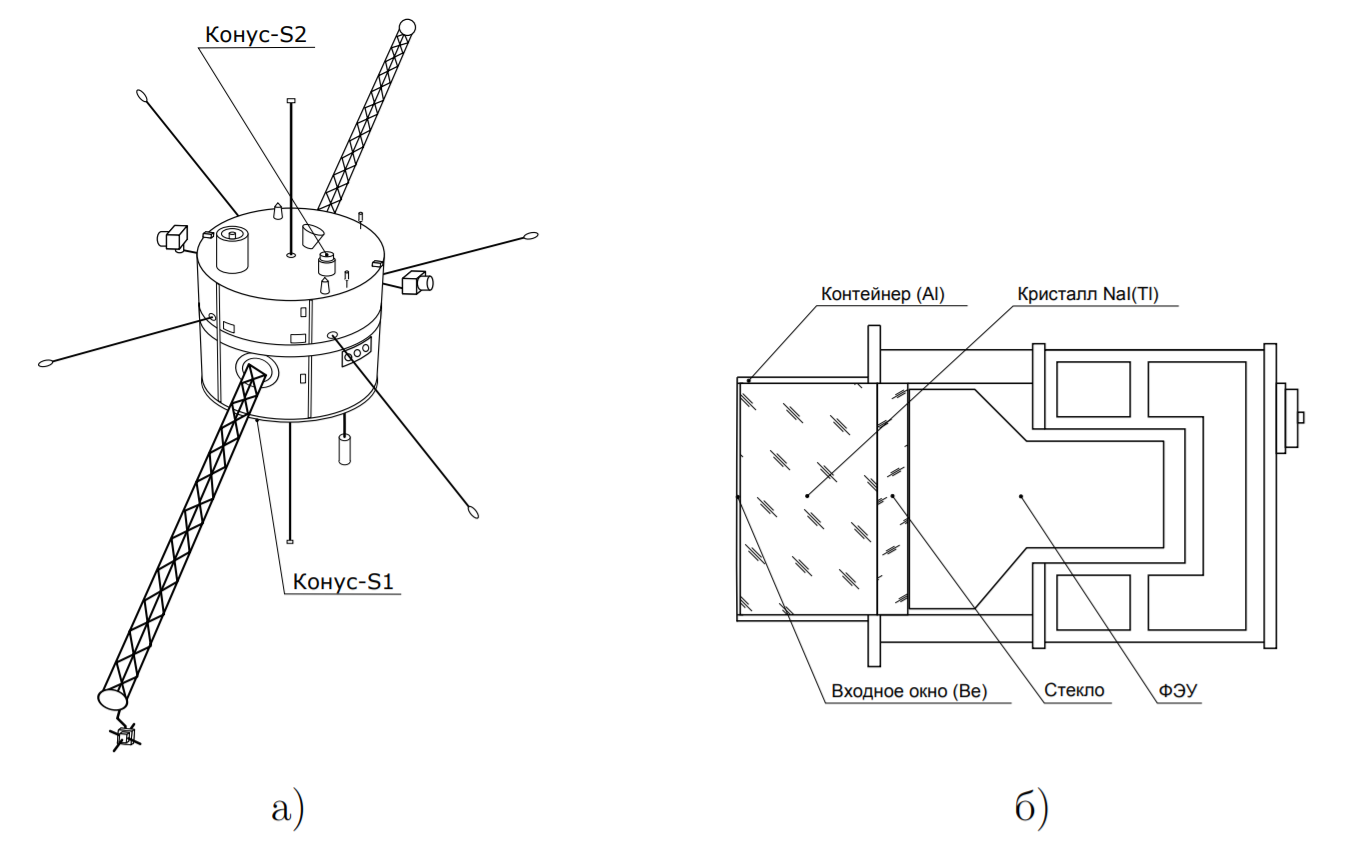
\includegraphics[width = 0.75\linewidth]{pictures/Konus-Wind.png}
		\caption{Устройство (а) спутника \textit{GGS-Wind} и (б) самого прибора}
		\label{img:kw1}
	\end{figure}
	
	BAT --- один из инструментов орбитальной обсерватории SWIFT, представляющий из себя телескоп с кодирующей маской. Кодирующая апертура является одним из способов построения изображения источника в жестком рентгеновском и мягком гамма диапазоне без использования системы линз и зеркал. Метод широко применяется в гамма- и рентген-астрономии, в том числе и в INTEGRAL/ISGRI. Линзы и зеркала в астрономии высоких энергий не используются, поскольку при попадании на линзу они почти не преломляются и либо проходят насквозь стекло, либо поглощаются материалом. Сигнал регистрирует массив CdZnTe-детекторов, половина которых закрывается маской. В отличие от Konus-Wind, его поле зрения меньше и равняется $1.4$ стерадиана. На рис. \ref{img:bat1} можно увидеть схематическое представление прибора.
	 
	 CdZnTe-детекторы также, как и CdZn являются полупроводниковыми детекторам, широко использующиеся в астрономии высоких энергий. Полупроводниковые детекторы представляют собой полупроводниковый кристалл и работает аналогично ионизационной камере. Главное их отличие состоит в том, что в камере используется газ, который является менее плотным, чем кристалл, что делает камеру менее чувствительной. Полупроводниковый детектор представляет собой полупроводниковый диод, на который подается какое-то обратное напряжение. Заряженная частица, попадая в область, находящеюся рядом с границей p-n перехода, создает электроно-дырочные пары, которые под воздейтсвием электрического поля продвигаются к электродам полупроводникового детектора. В результате в цепи образзуется какой-то электрический импульс, который можно измерить и узнать энергию, прилетевшей частицы. 
	
	\begin{figure}[h!]
		\centering
			\begin{subfigure}[b]{0.49\linewidth}
			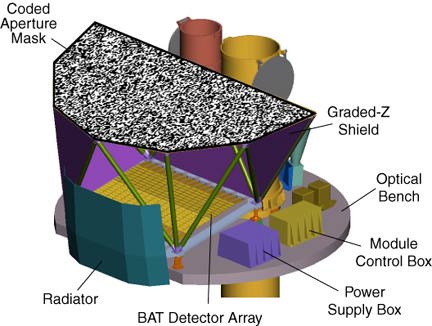
\includegraphics[width = \textwidth]{pictures/BAT.jpg}
			\caption{}
			\label{img:bat1}
		\end{subfigure}
		\begin{subfigure}[b]{0.49\linewidth}
		\centering
			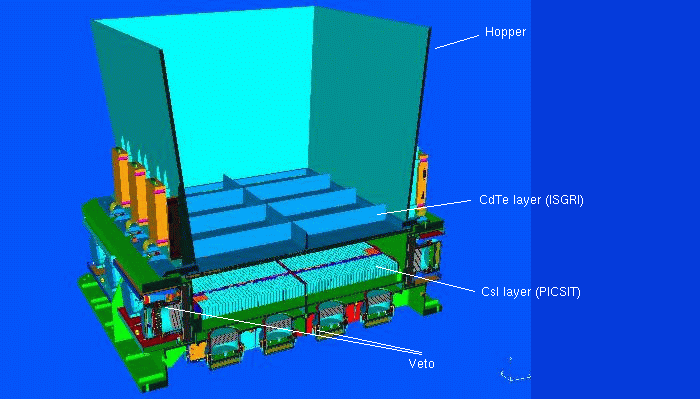
\includegraphics[width = \textwidth]{pictures/INTEGRAL.png}
			\caption{}
			\label{img:int1}
		\end{subfigure}
		\caption{Устройство прибора (a) BAT и (b) IBIS, частью которого является ISGRI}
	\end{figure}
	
	INTEGRAL аналогичен BAT, но его инструмент ISGRI импользует CdTe-детекторы и его поле зрения равно $0.26$ стерадиан. На рис. \ref{img:int1} представлено его схематическое строение. 
